\documentclass[conference]{IEEEtran}
\usepackage{amsmath,amssymb}
\usepackage{cite}
\usepackage{booktabs}
\usepackage{array}
\usepackage{url}
\usepackage{xcolor}
\usepackage{tikz}
\usetikzlibrary{arrows.meta,positioning}

\definecolor{rulecolor}{rgb}{0.15,0.35,0.65}

\title{Tradeoff-Explicit Governance for Reliable Distributed Computing Systems}

\author{\IEEEauthorblockN{Anonymous Submission}}

\begin{document}
\maketitle

\begin{abstract}
Distributed computing systems routinely balance consistency, latency, durability, availability, and cost, yet many production failures occur because these tradeoffs remain implicit in defaults, configuration files, or local operational knowledge. This paper proposes a tradeoff-explicit governance framework for distributed systems. The framework represents system behavior through five policy planes: consistency, performance, caching, durability, and flow control. It further defines six design rules: explicitness, boundaries, reversibility, observability, governance, and robustness. The objective is to make operationally significant tradeoffs visible at design time, observable at runtime, and reversible during incidents. The methodology combines synthesis from distributed systems theory with a retrospective qualitative analysis of publicly documented outages. The analysis shows that recurring failures can be interpreted as violations of tradeoff visibility, bounded change, and policy-context observability. The proposed framework is intended for architects and operators of databases, message streaming systems, storage platforms, and compute orchestrators where competing objectives must be governed rather than hidden.
\end{abstract}

\begin{IEEEkeywords}
distributed systems, computing systems, reliability engineering, operational governance, tradeoff analysis, policy-driven architecture
\end{IEEEkeywords}

\section{Introduction}

Modern distributed computing systems are rarely limited by a single technical objective. A storage system may need strong consistency for financial records and low-latency eventual consistency for session data. A message broker may increase throughput by batching, but the same decision can increase visibility delay and recovery risk. A compute orchestrator may improve scheduling quality by evaluating more constraints, but that improvement can slow recovery after node failure. These decisions are not implementation details; they are operational tradeoffs.

The problem addressed in this paper is that such tradeoffs are often implicit. They are encoded in defaults, spread across configuration surfaces, or understood only by experienced operators. During incidents, implicit tradeoffs make it difficult to distinguish a software defect from an expected consequence of a selected policy. This increases diagnosis time, widens blast radius, and can cause silent semantic degradation, where a system continues returning responses while violating the guarantee users believe is active.

This paper proposes \textit{tradeoff-explicit governance}: a design framework in which operationally significant tradeoffs are represented as visible policy controls with documented effects, measurable signals, ownership, and rollback procedures. The framework is motivated by established results such as CAP~\cite{brewer2000cap,gilbert2002brewer}, PACELC~\cite{pacelc}, tunable consistency in Dynamo~\cite{dynamo}, and operational practices from site reliability engineering~\cite{sre}. Its contribution is to connect these ideas into a practical governance model for distributed computing systems.

The paper makes three contributions:
\begin{itemize}
    \item It defines tradeoff-explicit governance as a policy-based model for distributed system design and operation.
    \item It introduces five policy planes and six design rules that make tradeoffs visible, observable, and reversible.
    \item It evaluates the framework through retrospective analysis of public production incidents and maps the framework across common distributed system classes.
\end{itemize}

The work is positioned within the computational intelligence and computing track, especially computing architectures and systems, software engineering, networks, and reliable cloud-scale infrastructure.

\section{Related Work}

The CAP theorem established that consistency, availability, and partition tolerance cannot all be guaranteed simultaneously in an asynchronous distributed system~\cite{brewer2000cap,gilbert2002brewer}. Brewer later emphasized that real systems operate on a spectrum rather than through a simple ``two of three'' choice~\cite{brewer2012cap}. PACELC extends this reasoning by observing that systems also trade latency against consistency when partitions are absent~\cite{pacelc}.

Distributed databases and storage systems expose these tradeoffs in different ways. Dynamo uses quorum parameters to tune consistency and availability, while pushing conflict resolution to application logic~\cite{dynamo}. Bigtable demonstrates large-scale distributed storage design, while Spanner uses TrueTime to provide external consistency with specialized infrastructure~\cite{bigtable,spanner}. Consensus protocols such as Paxos and Raft provide agreement under failure, but they do not by themselves decide which guarantees a workload should require~\cite{lamport2001paxos,raft}.

Operational reliability work complements this theory. Site reliability engineering formalizes service-level objectives, error budgets, monitoring, and incident response~\cite{sre}. Human factors and safety engineering show that accidents often emerge from interacting design, organizational, and control failures rather than isolated technical defects~\cite{leveson,humanfactors}. The proposed framework builds on these ideas by treating tradeoff selection as a first-class operational governance problem.

\section{Problem Definition}

Let a distributed system $S$ consist of components $C=\{c_1,c_2,\ldots,c_n\}$ that communicate over a network to provide a unified service. Let $O=\{o_1,o_2,\ldots,o_m\}$ be measurable objectives such as consistency, latency, durability, availability, quality, and cost. A tradeoff exists when improving one objective under a configuration change $\Delta$ degrades another objective:
\begin{equation}
o_i(S+\Delta)>o_i(S) \quad \land \quad o_j(S+\Delta)<o_j(S).
\end{equation}

A tradeoff is \textit{implicit} when operators cannot observe, measure, or modify it without changing code, reverse-engineering configuration, or relying on undocumented knowledge. A system approaches \textit{tradeoff-explicitness} when each important tradeoff is represented by a policy control that is visible at runtime, documented, measurable, owned, and reversible where feasible.

The research question is therefore: \textit{How can distributed computing systems be designed so that unavoidable tradeoffs become explicit governance decisions rather than hidden operational risks?}

\section{Methodology}

The framework was developed through three steps. First, recurring tradeoffs were extracted from distributed systems theory, including CAP, PACELC, quorum replication, consensus, caching, and flow control. Second, these tradeoffs were grouped into policy planes that correspond to common operational control surfaces. Third, the resulting framework was evaluated qualitatively against publicly documented production incidents to test whether it explains failure mechanisms and identifies preventive controls.

The evaluation is retrospective rather than experimental. This is appropriate because the framework concerns governance and diagnosability across system classes, not the performance of a single algorithm. The evaluation criteria are:
\begin{itemize}
    \item whether a rule violation can be identified from the public incident description;
    \item whether the involved policy planes explain the observed failure propagation;
    \item whether the framework suggests a concrete prevention or mitigation mechanism.
\end{itemize}

\section{Framework}

The framework has two layers. The first layer is a set of policy planes that describe where tradeoffs occur. The second layer is a set of rules that govern how those policies are exposed and changed.

\subsection{Policy Planes}

\textbf{Consistency plane:} Defines freshness and ordering guarantees. Controls include read consistency, write consistency, staleness budget, quorum size, and conflict resolution. Stronger consistency improves correctness but increases coordination cost and tail latency.

\textbf{Performance plane:} Defines computation depth and resource use. Controls include timeout thresholds, retry limits, scheduling depth, query complexity, and parallelism. Deeper processing can improve quality but increases compute cost and latency.

\textbf{Caching plane:} Defines result reuse and invalidation. Controls include cache scope, time-to-live, eviction policy, and coherence strategy. Aggressive caching improves repeated-request latency but increases staleness and invalidation complexity.

\textbf{Durability plane:} Defines persistence posture. Controls include write acknowledgment level, write-ahead log flushing, replication synchronicity, checkpointing, and backup verification. Stronger durability reduces data-loss risk but can reduce write throughput.

\textbf{Flow-control plane:} Defines admission, batching, queues, and backpressure. Controls include queue depth, batch size, rate limits, circuit breakers, and admission rules. Flow control protects stability under load but can introduce delay or rejected traffic.

\begin{table}[t]
\caption{Policy Planes and Primary Tradeoffs}
\label{tab:planes}
\centering
\small
\begin{tabular}{@{}l l l@{}}
\toprule
\textbf{Plane} & \textbf{Improves} & \textbf{Can Degrade} \\
\midrule
Consistency & Correctness & Latency, availability \\
Performance & Quality, utilization & Cost, tail latency \\
Caching & Repeated-read speed & Freshness \\
Durability & Crash recovery & Write throughput \\
Flow control & Stability & Delay, acceptance rate \\
\bottomrule
\end{tabular}
\end{table}

\subsection{Design Rules}

\textbf{Rule 1: Explicitness.} Every critical guarantee and tradeoff must be declared. Consistency and durability should be specified per data product or workload rather than only per system.

\textbf{Rule 2: Boundaries.} Service boundaries must also define fault domains, ownership, and degradation paths. Control planes and data planes should be independently scalable, deployable, and recoverable.

\textbf{Rule 3: Reversibility.} Policy changes must be bounded in scope, testable, and reversible where feasible. Each change should have a rollback trigger and an expiry or review point.

\textbf{Rule 4: Observability.} Metrics must be displayed with active policy context. A latency spike, replication delay, or cache hit-rate change is not fully interpretable unless operators know which policy profile is active.

\textbf{Rule 5: Governance.} Each policy plane needs ownership. Policy changes should document objective, known downside, expected signal movement, and rollback trigger.

\textbf{Rule 6: Robustness.} If a system cannot preserve declared semantics under stress, it should fail explicitly with identifiable error information rather than silently returning degraded results.

\begin{figure}[t]
\centering
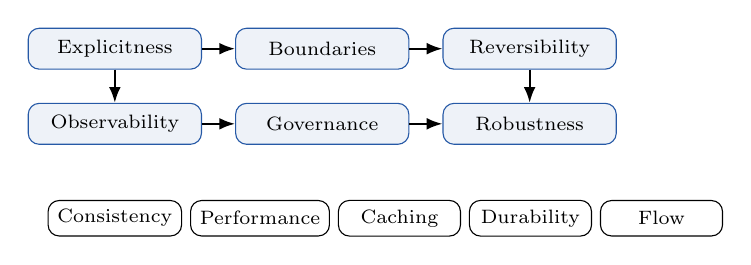
\begin{tikzpicture}[
    node distance=0.42cm,
    rule/.style={rectangle, draw=rulecolor, fill=rulecolor!8, rounded corners,
    minimum width=2.2cm, minimum height=0.52cm, align=center, font=\scriptsize},
    plane/.style={rectangle, draw, rounded corners, minimum width=1.55cm,
    minimum height=0.45cm, align=center, font=\scriptsize},
    arrow/.style={-{Latex[length=2mm]}, thick}
]
\node[rule] (r1) {Explicitness};
\node[rule, right=of r1] (r2) {Boundaries};
\node[rule, right=of r2] (r3) {Reversibility};
\node[rule, below=of r1] (r4) {Observability};
\node[rule, right=of r4] (r5) {Governance};
\node[rule, right=of r5] (r6) {Robustness};
\draw[arrow] (r1) -- (r2);
\draw[arrow] (r2) -- (r3);
\draw[arrow] (r1) -- (r4);
\draw[arrow] (r4) -- (r5);
\draw[arrow] (r5) -- (r6);
\draw[arrow] (r3) -- (r6);
\node[plane, below=0.7cm of r4] (p1) {Consistency};
\node[plane, right=0.1cm of p1] (p2) {Performance};
\node[plane, right=0.1cm of p2] (p3) {Caching};
\node[plane, right=0.1cm of p3] (p4) {Durability};
\node[plane, right=0.1cm of p4] (p5) {Flow};
\end{tikzpicture}
\caption{Tradeoff-explicit governance combines six design rules with five operational policy planes.}
\label{fig:framework}
\end{figure}

\subsection{Decision Calculus}

For a workload, each policy profile $p$ can be scored across objectives: consistency ($C_p$), latency ($L_p$), durability ($D_p$), quality ($Q_p$), and cost efficiency ($E_p$). Scores are normalized to $[0,1]$. A workload selects:
\begin{equation}
p^*=\arg\max_p \sum_{j\in\{C,L,D,Q,E\}} w_j j_p
\end{equation}
subject to guardrails such as maximum p99 latency or minimum durability. This calculus does not replace engineering judgment; it makes disagreement explicit. Teams debate weights and guardrails instead of hidden assumptions.

\section{Retrospective Evaluation}

Table~\ref{tab:evaluation} maps four public incidents to the proposed rules. The purpose is not to claim full causal access to private systems, but to test whether the framework identifies visible governance failures in published reports.

\begin{table}[t]
\caption{Retrospective Mapping of Public Incidents}
\label{tab:evaluation}
\centering
\small
\begin{tabular}{@{}p{1.15cm}p{1.65cm}p{3.05cm}@{}}
\toprule
\textbf{Case} & \textbf{Main Planes} & \textbf{Framework Interpretation} \\
\midrule
GitHub 2018~\cite{github2018} & Consistency, durability & Replica lag and failover state required clearer policy visibility and rollback semantics. \\
GitLab 2017~\cite{gitlab2017} & Durability, observability & Backup and replication guarantees were not sufficiently visible or continuously validated. \\
AWS S3 2017~\cite{aws2017} & Flow control, boundaries & A bounded operational action propagated through insufficiently isolated subsystems. \\
Cloudflare 2020~\cite{cloudflare2020} & Flow control, governance & Configuration propagation needed stronger staged rollout, signal expectations, and rollback rules. \\
\bottomrule
\end{tabular}
\end{table}

Across the cases, three patterns recur. First, policy state was not sufficiently explicit at the moment operators needed to reason about the system. Second, changes had large blast radius or weak rollback triggers. Third, metrics were difficult to interpret without the policy context that produced them. These patterns correspond directly to Rules 1, 3, and 4.

The framework also explains cross-plane interaction. In database failover, durability posture and replication delay affect consistency. In global configuration deployment, flow-control policy affects performance and availability. In backup failures, observability determines whether durability claims are trustworthy. Thus, incidents are rarely confined to a single plane; they emerge from unmanaged interaction between planes.

\section{Application Across System Types}

\textbf{Distributed databases:} The framework requires consistency and durability to be declared per workload. For example, a ledger can require strict reads and synchronous replication, while a session store can use bounded staleness with lower cost. The same database should not hide both requirements behind one global default.

\textbf{Message streaming systems:} Ordering, acknowledgment, replication, and batching can be expressed as policy planes. A producer acknowledgment change should include expected throughput improvement, durability downside, monitoring signals, and rollback trigger.

\textbf{Storage systems:} Replication factor, read-after-write semantics, cache invalidation, and backup verification are made explicit. If a declared backup guarantee is not being met, Rule 6 requires explicit failure or alerting rather than silent confidence.

\textbf{Compute orchestrators:} Scheduling depth, admission control, pod eviction, and control-plane load are governed as policies. A scheduler can trade placement optimality for failover speed, but the selected profile and its expected effect must be visible.

\section{Discussion}

Tradeoff-explicit governance introduces overhead. It increases the policy surface that teams must document and maintain. It also risks overwhelming operators if too many low-level controls are exposed. The framework therefore favors intent-oriented profiles over raw parameter exposure. The aim is not to expose every internal knob; it is to expose every decision that changes user-visible guarantees or operational risk.

The framework is limited by its qualitative evaluation. Future work should implement policy linting and policy-context dashboards in a real distributed platform, then measure incident diagnosis time, rollback time, and operator error rates before and after adoption. Another direction is tenant-aware governance, where different tenants require different policy profiles within the same shared infrastructure.

\section{Conclusion}

Distributed systems cannot avoid tradeoffs, but they can avoid hiding them. This paper presented a tradeoff-explicit governance framework based on five policy planes and six design rules. The framework converts hidden operational assumptions into visible, measurable, owned, and reversible policy decisions. Retrospective analysis of public incidents suggests that many failures involve exactly the problems the framework targets: implicit guarantees, unbounded changes, missing policy context, and silent semantic degradation. By making tradeoffs explicit, distributed computing systems can become easier to operate, audit, and recover under stress.

\begin{thebibliography}{00}

\bibitem{brewer2000cap}
E. A. Brewer, ``Towards robust distributed systems,'' in \textit{Proc. ACM PODC}, 2000.

\bibitem{gilbert2002brewer}
S. Gilbert and N. Lynch, ``Brewer's conjecture and the feasibility of consistent, available, partition-tolerant web services,'' \textit{ACM SIGACT News}, vol. 33, no. 2, pp. 51--59, 2002.

\bibitem{pacelc}
D. J. Abadi, ``Consistency tradeoffs in modern distributed database system design,'' \textit{IEEE Computer}, vol. 45, no. 2, pp. 37--42, 2012.

\bibitem{dynamo}
G. DeCandia et al., ``Dynamo: Amazon's highly available key-value store,'' in \textit{Proc. ACM SOSP}, 2007.

\bibitem{bigtable}
F. Chang et al., ``Bigtable: A distributed storage system for structured data,'' in \textit{Proc. USENIX OSDI}, 2006.

\bibitem{spanner}
J. C. Corbett et al., ``Spanner: Google's globally distributed database,'' in \textit{Proc. USENIX OSDI}, 2012.

\bibitem{lamport2001paxos}
L. Lamport, ``Paxos made simple,'' \textit{ACM SIGACT News}, vol. 32, no. 4, pp. 18--25, 2001.

\bibitem{raft}
D. Ongaro and J. Ousterhout, ``In search of an understandable consensus algorithm,'' in \textit{Proc. USENIX ATC}, 2014.

\bibitem{sre}
B. Beyer et al., \textit{Site Reliability Engineering}. O'Reilly Media, 2016.

\bibitem{leveson}
N. G. Leveson, \textit{Engineering a Safer World}. MIT Press, 2011.

\bibitem{humanfactors}
S. Dekker, \textit{The Field Guide to Understanding Human Error}, 3rd ed. CRC Press, 2014.

\bibitem{brewer2012cap}
E. A. Brewer, ``CAP twelve years later: How the rules have changed,'' \textit{IEEE Computer}, vol. 45, no. 2, pp. 23--29, 2012.

\bibitem{github2018}
GitHub Engineering, ``Incident report: Database failover on October 21, 2018,'' 2018. [Online]. Available: \url{https://github.blog/2018-10-30-oct21-incident-report/}

\bibitem{gitlab2017}
GitLab, ``GitLab.com database incident,'' 2017. [Online]. Available: \url{https://about.gitlab.com/2017/02/01/gitlab-dot-com-database-incident/}

\bibitem{aws2017}
Amazon Web Services, ``Summary of the Amazon S3 service disruption in the US-EAST-1 region,'' 2017. [Online]. Available: \url{https://aws.amazon.com/message/41926/}

\bibitem{cloudflare2020}
Cloudflare, ``Cloudflare outage on June 24, 2020,'' 2020. [Online]. Available: \url{https://blog.cloudflare.com/cloudflare-outage-on-june-24-2020/}

\end{thebibliography}

\end{document}
